% !TeX spellcheck = de_CH
%%%%%%%%%%%%%%%%%%%%%%%%%%%%%%%%%%%%%%%%%%%%%%%%%%%%%%%%%%%%%%%%%
%  _____   ____  _____                                          %
% |_   _| /  __||  __ \    Institute of Computitional Physics   %
%   | |  |  /   | |__) |   Zuercher Hochschule Winterthur       %
%   | |  | (    |  ___/    (University of Applied Sciences)     %
%  _| |_ |  \__ | |        8401 Winterthur, Switzerland         %
% |_____| \____||_|                                             %
%%%%%%%%%%%%%%%%%%%%%%%%%%%%%%%%%%%%%%%%%%%%%%%%%%%%%%%%%%%%%%%%%
%
% Project     : BA Welti Keller
% Title       : 
% File        : hardware.tex Rev. 00
% Date        : 15.09.2014
% Author      : Tobias Welti
%
%%%%%%%%%%%%%%%%%%%%%%%%%%%%%%%%%%%%%%%%%%%%%%%%%%%%%%%%%%%%%%%%%

\chapter{Hardware-Konzept}\label{chap.hardware}



\section{Hardware-Architektur}\label{sec.hw_arch}

Anhand der funktionalen Vorgaben für die Messstation werden der \gls{logger}, die \gls{sensoreinh} und das Bussytem im folgenden genauer spezifiziert und die Komponenten ausgewählt.

\subsection{Datenlogger}
Das \gls{hardware}-Konzept des \gls{logger}s ist in Abbildung \ref{fig.hwkonzept_logger} dargestellt.
Der \gls{logger} sammelt die Daten der \glspl{sensoreinh} über das \gls{bussys} ein und speichert sie ab. Dafür benötigt er das \gls{bussys}, einen Mikroprozessor, internen Speicher und ein leicht auswechselbares \gls{speichermedium}. Ausserdem soll über eine Schnittstelle ein Computer angeschlossen werden können, um den Betrieb der Messstation zu steuern. Der \gls{logger} wird in einem wasserdichten Gehäuse untergebracht. Für den Austausch des \gls{speichermedium}s wäre eine verschraubbare Öffnung denkbar.

\begin{figure}[H]
	\centering
		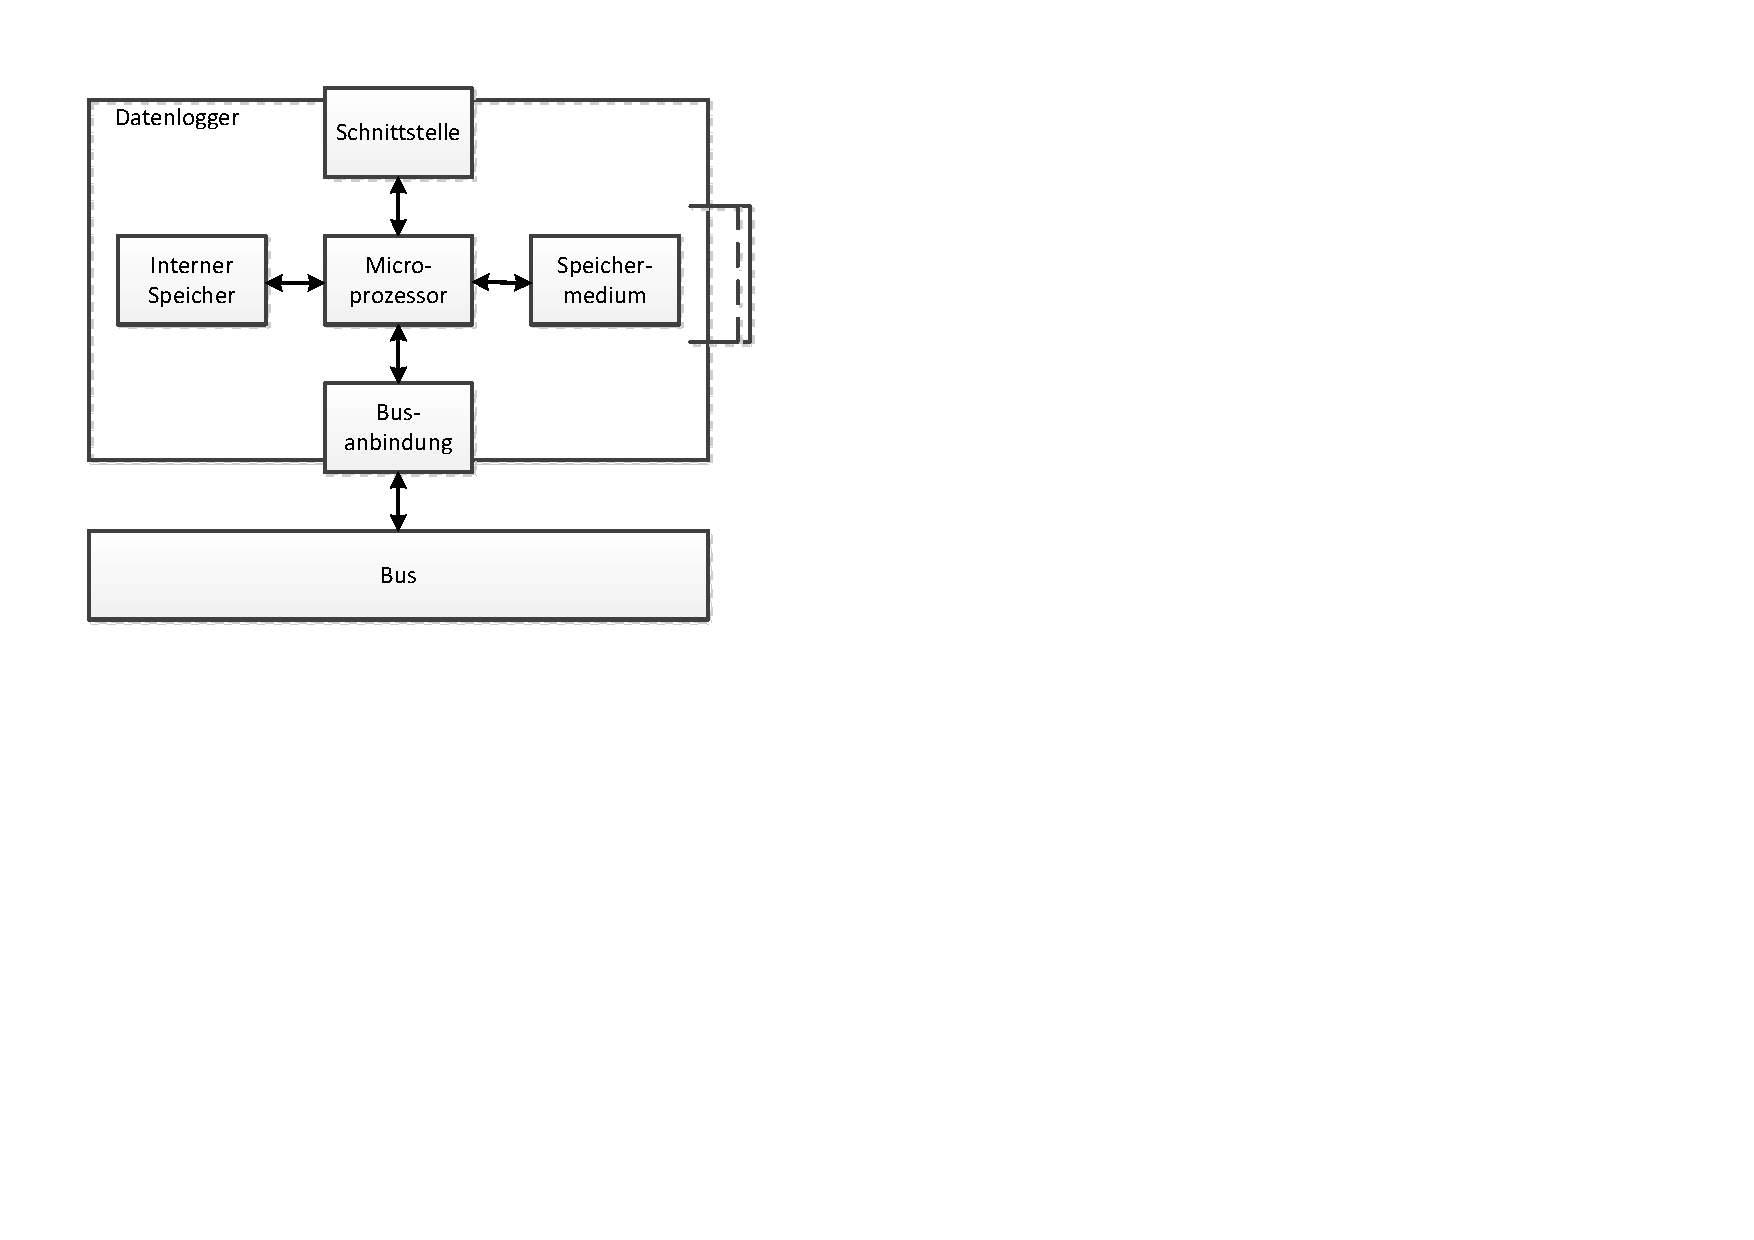
\includegraphics[width=0.8\textwidth]{images/visio/hardwarekonzept_logger.pdf}
	\caption{Hardwarekonzept des \gls{logger}s.}
	\label{fig.hwkonzept_logger}
\end{figure}

\subsection{Sensoreinheit}
Die \gls{sensoreinh} benötigt einen Beschleunigungssensor, um die Einschläge von Geschiebe zu messen. Über einen Analog-Digital-Wandler (ADC) werden die Messsignale digitalisiert. Die gemessenen Signale werden von einem Mikroprozessor verarbeitet, im internen Speicher zwischengespeichert und über das \gls{bussys} an den \gls{logger} übertragen. Abbildung \ref{fig.hwkonzept_sensor} zeigt das \gls{hardware}-Konzept der \gls{sensoreinh}.

\begin{figure}[H]
	\centering
		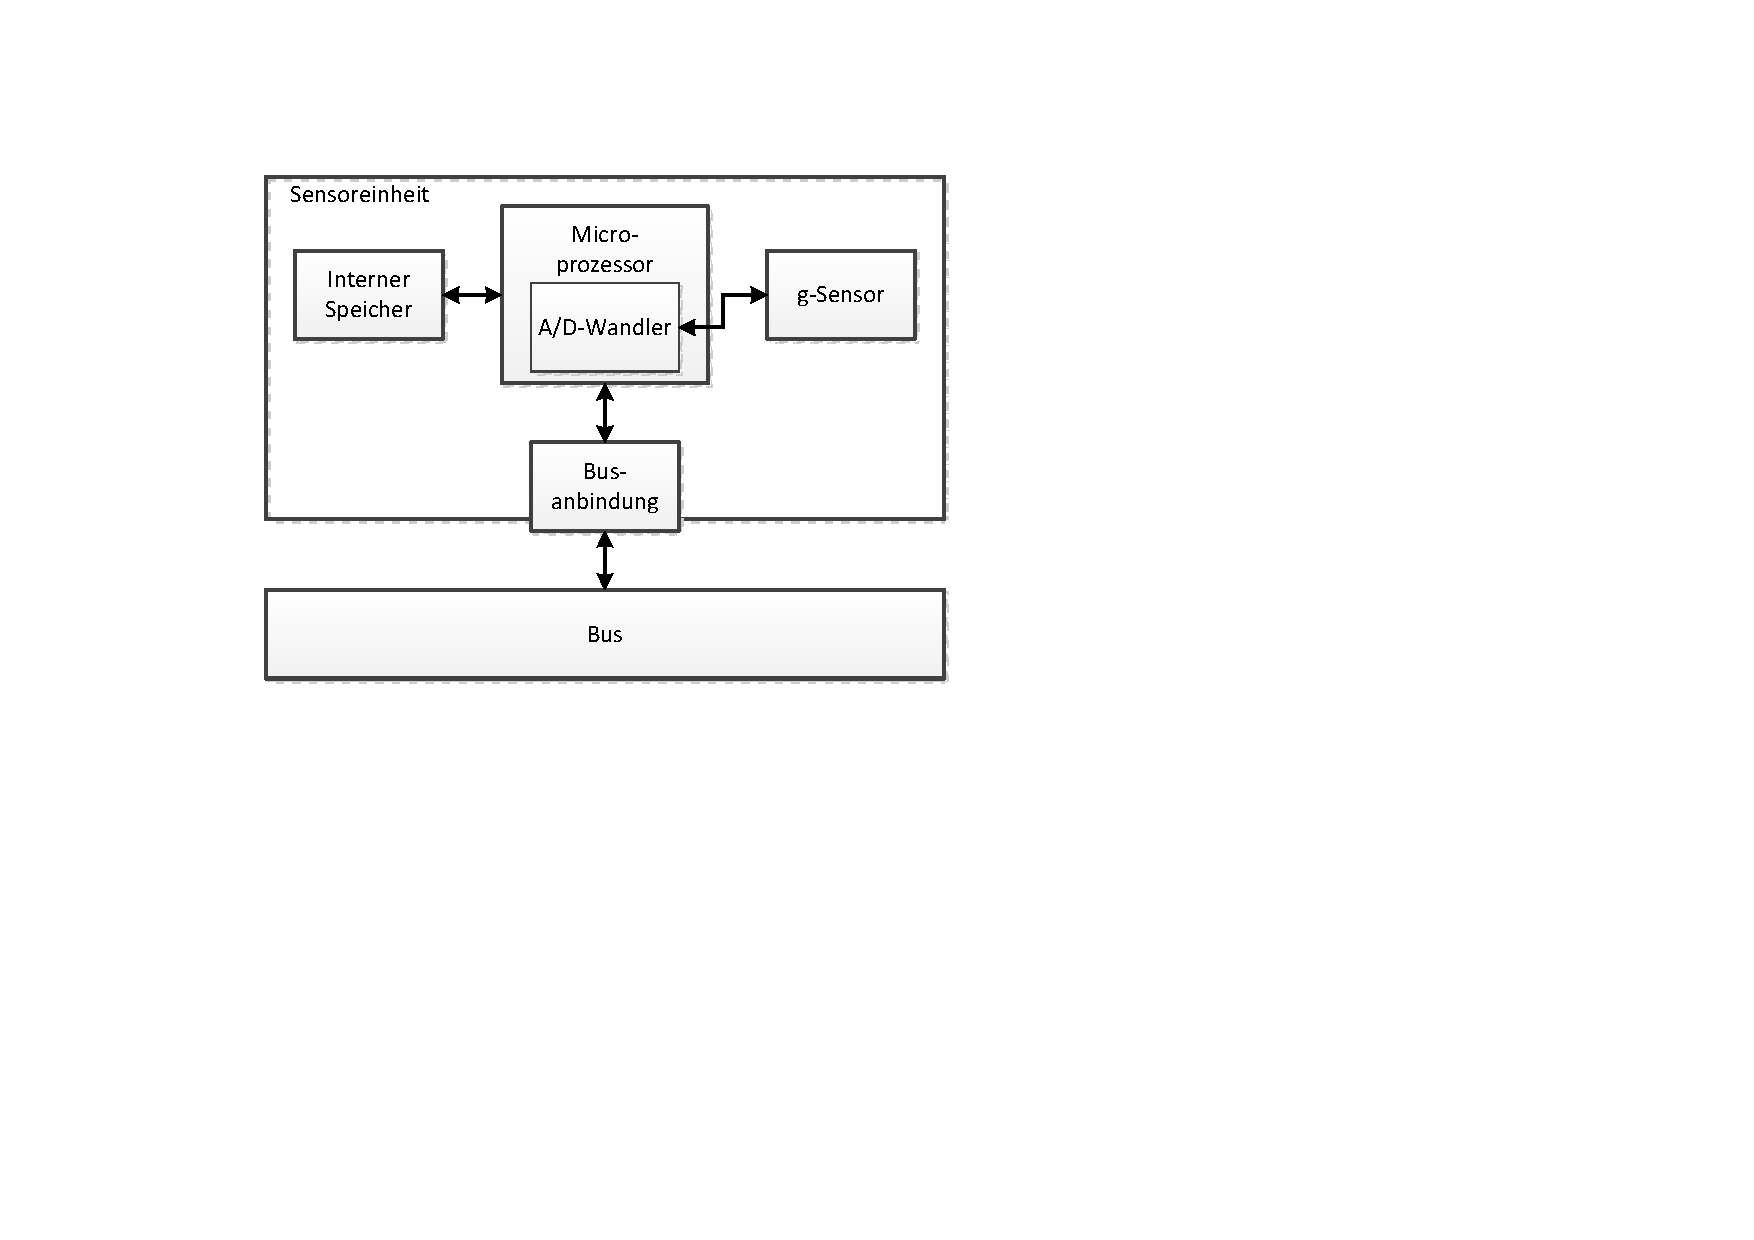
\includegraphics[width=0.8\textwidth]{images/visio/hardwarekonzept_sensor.pdf}
	\caption{Hardwarekonzept der \gls{sensoreinh}.}
	\label{fig.hwkonzept_sensor}
\end{figure}

\subsection{\gls{bussys}}
Das \gls{bussys} muss die Daten und Befehle zwischen \gls{logger} und \glspl{sensoreinh} übertragen. Die Reichweite des \gls{bussys}s muss genügen, um alle Komponenten der Messinstallation zu verbinden. Die Datenbandbreite muss die Übertragung der Messresultate aller \glspl{sensor} erlauben.


\section{Komponentenauswahl}

\subsection{Mikroprozessor}
Bei der Auswahl des Mikroprozessors werden folgende Kriterien berücksichtigt:

\begin{itemize}
\item Rechenleistung genügend für allfällige zusätzliche Anforderungen.
\item Analog-Digital-Wandler mit genügender Abtastrate und Auflösung.
\item Digitaler Signal Prozessor integriert für die Verarbeitung der Messdaten.
\item Ein-/Ausgänge für das \gls{bussys}.
\item Ein-/Ausgänge für den externen Speicher.
\item möglichst geringer Stromverbrauch.
\end{itemize}



\subsection{Bus-System}
Anhand folgender Kriterien wurde ein \gls{bussys} ausgewählt:

\begin{itemize}
\item Übertragungsbandbreite genügend für fortlaufende Übertragung von Rohdaten einer \gls{sensoreinh}.
\item Reichweite mindestens 20 Meter.
\item Robust gegenüber äusseren Einflüssen.
\item Mindestens zwanzig Busteilnehmer möglich.
\end{itemize}

\begin{table}
\begin{tabular}{|l|l|l|l|l|}
\hline  & \textbf{Bitrate}      & \textbf{Distanz} & \textbf{Clients} & \textbf{Besonderheiten}\\ 
\hline \textbf{CAN} & \begin{minipage}{2cm}
1 MBit/s\\ 125 kBit/s
\end{minipage} & \begin{minipage}{1.5cm}40 m\\500 m\end{minipage} & > 20 & \begin{minipage}{6cm}
\mbox{ }\\+ Collision Detection (CD) umgehen mit Polling durch Master.\\
+ Bei synchronem CAN wird CD durch ID gelöst.\\
+ CAN Controller sendet Interrupt Request bei erhaltener Nachricht.\\
\end{minipage} \\ 
\hline \textbf{SPI} & ..100 MBit/s & < 1 m & \begin{minipage}{1cm}
slave select
\end{minipage} & \begin{minipage}{6cm}
\mbox{ }\\- Pro Client eine Slave Select Leitung\\
- Daisy Chain $\Rightarrow $alle MC beschäftigt.\\
- Bei Ausfall eines MC ganzer Bus unterbrochen.\\
\end{minipage} \\ 
\hline \textbf{RS485} & \begin{minipage}{2cm}
35 MBit/s\\100 kBit/s
\end{minipage} & \begin{minipage}{1.5cm}
10 m\\1200 m
\end{minipage} & >32 & \begin{minipage}{6cm}
\mbox{ }\\- Master am besten in der Mitte des Bus $\Rightarrow$ ungünstig.\\
- Braucht 2..4 Drähte (bei Full Duplex)\\
- braucht pull-up und pull-down Widerstände $\Rightarrow$ mehr Leistungsaufnahme.\\
\end{minipage} \\ 
\hline \textbf{Ethernet} & 100 MBit/s & 100 m & > 20 & \begin{minipage}{6cm}
\mbox{ }\\+ Stromversorgung bei Power over Ethernet (PoE) integriert.\\
- kein Bus sondern allenfalls Daisychain.\\
- bei Daisychain kein PoE möglich.\\
\end{minipage} \\ 
\hline \textbf{Feldbus} &  &  &  & \begin{minipage}{6cm}
\mbox{ }\\ist eine Familie von Bussen, z.B. CAN-Bus\\
\end{minipage} \\ 
\hline \textbf{I2C} & 0.4..5 Mbit/s & wenige Meter & < 20 & \begin{minipage}{6cm}
\mbox{ }\\nur für kurze Distanzen, Bitrate nimmt rasch ab.\\
\end{minipage}\\
\hline 
\end{tabular}
\caption{Entscheidungsmatrix für die Auswahl des \gls{bussys}s.}
\label{table.bussystem}
\end{table} 

In Tabelle \ref{table.bussystem} sind die Eigenschaften diverser \glspl{bussys} aufgeführt.

\paragraph{Kommentare}
SPI und I2C sind nur für kurze Distanzen geeignet und sind deshalb keine Option.
Die Verwendung von Ethernet zur Datenübertragung würde zwei Schnittstellen auf jeder \gls{sensoreinh} voraussetzen, um die \glspl{sensor} hintereinander zusammenzuhängen (Daisychain). Jedes Paket müsste vom Microcontroller weitergeleitet werden, wenn es für einen anderen Empfänger bestimmt ist. Dies führte zu einer zusätzlichen Belastung der Microcontroller. Stromversorgung über Ethernet ist mit PowerOverEthernet (PoE) zwar möglich, erfordert aber spezielle Geräte zur Speisung über den Stecker des Datenkabels. Dies verunmöglicht eine Daisychain mit PoE, neben dem Datenkabel wäre noch ein Kabel für die Stromversorgung notwendig.

\paragraph{Vergleich CAN-Bus und RS485}
\todo{Kriterienliste RS485/CAN einfügen, Lit-Referenz auf White Paper von IXXAT}
CAN und RS: Stecker nicht definiert => wasserdichte Stecker einfach zu finden.

\paragraph{Entscheidung}
CAN-Bus erfüllt alle Kriterien und erlaubt es, den Busmaster am Ende des Bus zu platzieren. Dies ist ein Vorteil gegenüber RS485, wo der Master in der Mitte platziert werden sollte. CAN-Bus bietet bereits Kollisionserkennung und Fehlererkennung, während dies bei RS485 in der Software gelöst werden muss. Für CAN-Bus sind Bus-Treiber (Transceiver) erhältlich, die mit hohen Spannungen umgehen können, was das \gls{bussys} robuster gegenüber Umwelteinflüssen macht. Die Grösse der Datenpakete ist bei CAN-Bus auf 8 Byte begrenzt, bei RS485 werden die Datenpakete über die Software frei definiert, was ein klarer Vorteil von RS485 darstellt. Insgesamt überwiegen die Vorteile von CAN-Bus klar. 



\subsection{Speichermedium}
\paragraph{Kriterien} Das externe Speichermedium soll möglichst klein sein, wenig Stromverbrauch haben und einfach auswechselbar sein. Bei Inaktivität sollte das Medium wenn möglich keinen Strom verbrauchen. Für einen mehrwöchigen unabhängigen Betrieb einer Messstation muss genügend Speicherkapazität bereitgestellt werden.

\paragraph{Datenmenge} Pro \gls{sensor} werden bei hohem Geschiebeaufkommen maximal hundert \glspl{ereignis} pro Sekunde erwartet. Ein solches Geschiebeaufkommen stellt jedoch die Ausnahme dar. Ein \gls{ereignis} benötigt je nach verlangtem Detailgrad und Dauer des \gls{ereignis}ses 10..90 Byte Speicherplatz. Für den normalen Betriebsmodus werden 50 Byte/\gls{ereignis} gerechnet, bei 5 \glspl{ereignis}n pro Sekunde. Damit ergibt sich eine Datenrate von 250 Byte/s, die es pro \gls{sensor} abzuspeichern gilt. Mit zehn \glspl{sensor} im Einsatz müssen 2.5 kByte/s gespeichert werden. 

\paragraph{Unabhängige Betriebsdauer} Pro Gigabyte Speicherplatz können 111 Stunden Daten für zehn \glspl{sensor} gespeichert werden. Bei hohem Geschiebeaufkommen mit zwanzig mal mehr \glspl{ereignis}n bleiben immer noch 5 Stunden Aufzeichnungszeit pro Gigabyte. Begnügt man sich mit weniger Details, reichen fallen pro \gls{sensor} in zehn Sekunden rund 400 Byte Daten an. Bei dieser Datenrate reicht ein Gigabyte für rund 700 Stunden. Auch bei hohem Geschiebeaufkommen kann die Anlage mehrere Tage an Daten speichern. 

\paragraph{Kapazität} Heute sind Speichermedien mit Kapazitäten bis über 128 GB erhältlich, so dass die Detailrate kein entscheidendes Kriterium mehr darstellt.

\paragraph{Datentransfer} Für den Transfer der Daten aus dem \gls{logger} auf einen Computer gibt es grundsätzlich zwei Varianten. Entweder man liest die Daten über eine Schnittstelle auf den Computer aus, oder man tauscht das Speichermedium aus. Das Auslesen via Schnittstelle benötigt zusätzlich Strom, das Wechseln des Speichermediums setzt einen mehr oder weniger komfortablen und trotzdem wasserdichten Zugang zum Medium voraus. Da heute Speichermedien mit kleinem Platzbedarf erhältlich sind, könnte ein solcher Zugang recht einfach mit einem Schraubverschluss realisiert werden.

\paragraph{Vergleich} In Tabelle \ref{table.speichermedium} werden verschiedene Speichermedien miteinander verglichen. In der Spalte 'Breite' ist aufgelistet, wie gross eine Öffnung mindestens sein muss, um das Speichermedium wechseln zu können. 'Pins' gibt an, wie viele Leitungen für den Anschluss des Mediums am Microcontroller nötig sind. Der Stromverbrauch in Klammern ist für den Standby-Modus des Speichermediums.

\begin{table}
\begin{tabular}{|l|l|l|l|l|}
	\hline
	                      & \textbf{Breite} & \textbf{Pins} & \textbf{Stromverbrauch} & \textbf{Bemerkungen}        \\ \hline
	\textbf{SD-Card}      & 24 mm           & 9             & 20..100 mA (0.2 mA)     & 4 bit breiter serieller Bus \\ \hline
	\textbf{CompactFlash} & 43 mm           & 50            & max. 70 mA (k.A.)       & paralleler Bus              \\ \hline
	\textbf{USB-Stick}    & min. 12 mm      & 4             & typ. 70 mA (k.A.) &  \\ \hline
\end{tabular} 
\caption{Entscheidungsmatrix zur Auswahl des Speichermediums.}
\label{table.speichermedium}
\end{table} 

\todo{Literatur-Referenzen in Tabelle \ref{table.speichermedium}}


\paragraph{Entscheid} Für einen verschraubbaren Verschluss ist die CompactFlash-Karte zu breit, das Gehäuse würde dadurch sehr gross werden. Die SD-Karte und der USB-Stick sind vergleichbar in der Grösse. Von der SD-Karte sind auch kleinere Varianten erhältlich. Eine Öffnung für den Austausch des Speichermediums kann eine gewisse Grösse ohnehin nicht unterschreiten, damit hineingegriffen werden kann. Da die SD-Karte im Standby den geringeren Stromverbrauch hat, wird der \gls{logger} mit einem SD-Kartenleser ausgestattet.

\subsection{Sensor}
\todo{Sensorauswahl beschreiben}

\subsection{Schnittstelle}
\todo{Schnittstellenauswahl beschreiben}



\section{Komponenten}
\todo{Texten}
\subsection{Cortex M4 Mikroprozessor}

\todo{Cortex M4 beschreiben}
\subsubsection{Flash Speicher}

\todo{Flash Speicher beschreiben}
\subsubsection{SDRAM}

\todo{SDRAM beschreiben}

\subsection{Beschleunigungs-Sensor}

\todo{Sensor beschreiben}
\subsection{CAN Bus}

\todo{CAN Bus beschreiben}
\subsubsection{CAN Transceiver}

\todo{CAN Transceiver beschreiben}

\subsection{SD Karte}

\todo{SD-Karte/MCI beschreiben}
\subsection{UART Schnittstelle}

\todo{UART beschreiben}

\subsection{Gehäuse}
\todo{Gehäuse beschreiben}
\section{Datenlogger}

\todo{Datenlogger übersicht}
\begin{figure}[H]
	\centering
		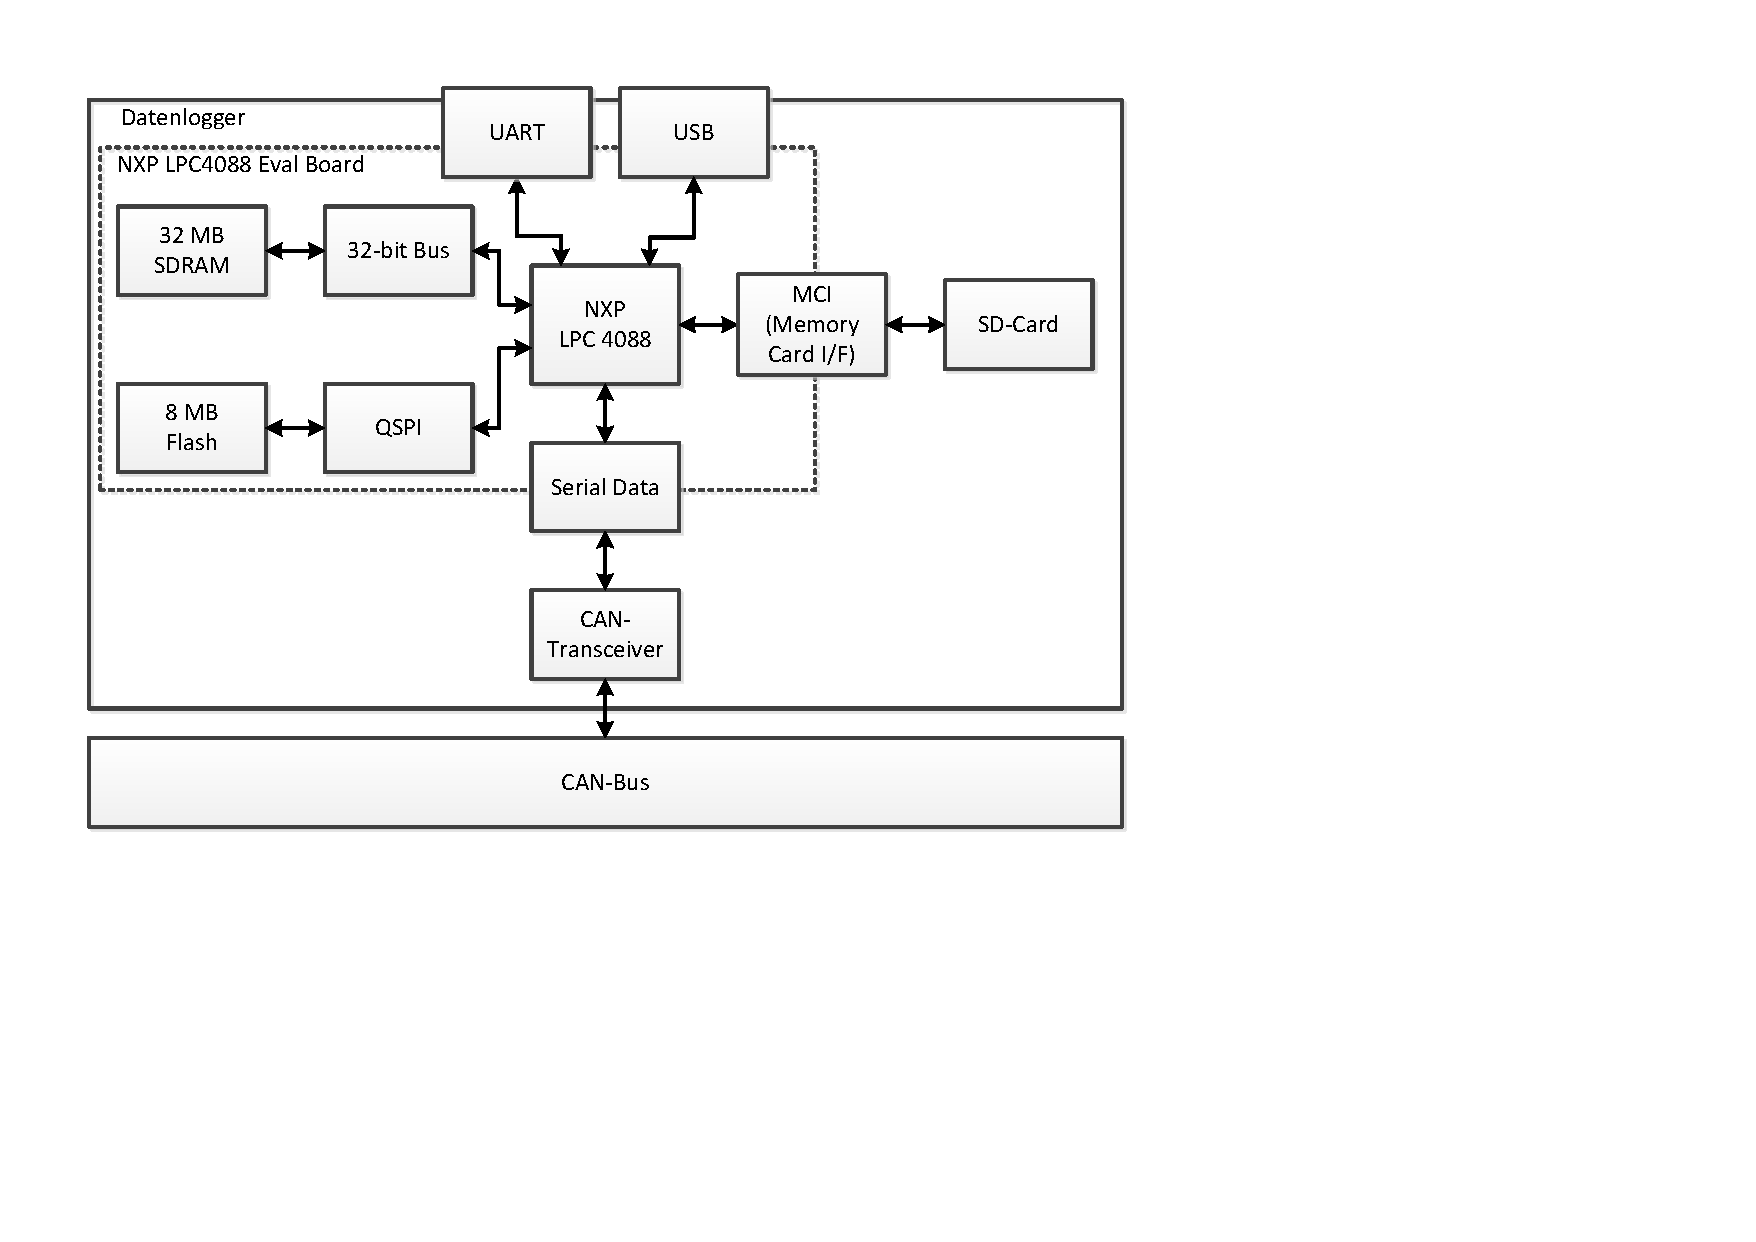
\includegraphics[width=0.8\textwidth]{images/visio/hardware_logger.pdf}
	\caption{Schematischer Hardware-Aufbau des \gls{logger}s.}
	\label{fig.hw_logger}
\end{figure}



\section{Sensoreinheit}

\todo{Sensoreinheit übersicht}
\begin{figure}[H]
	\centering
		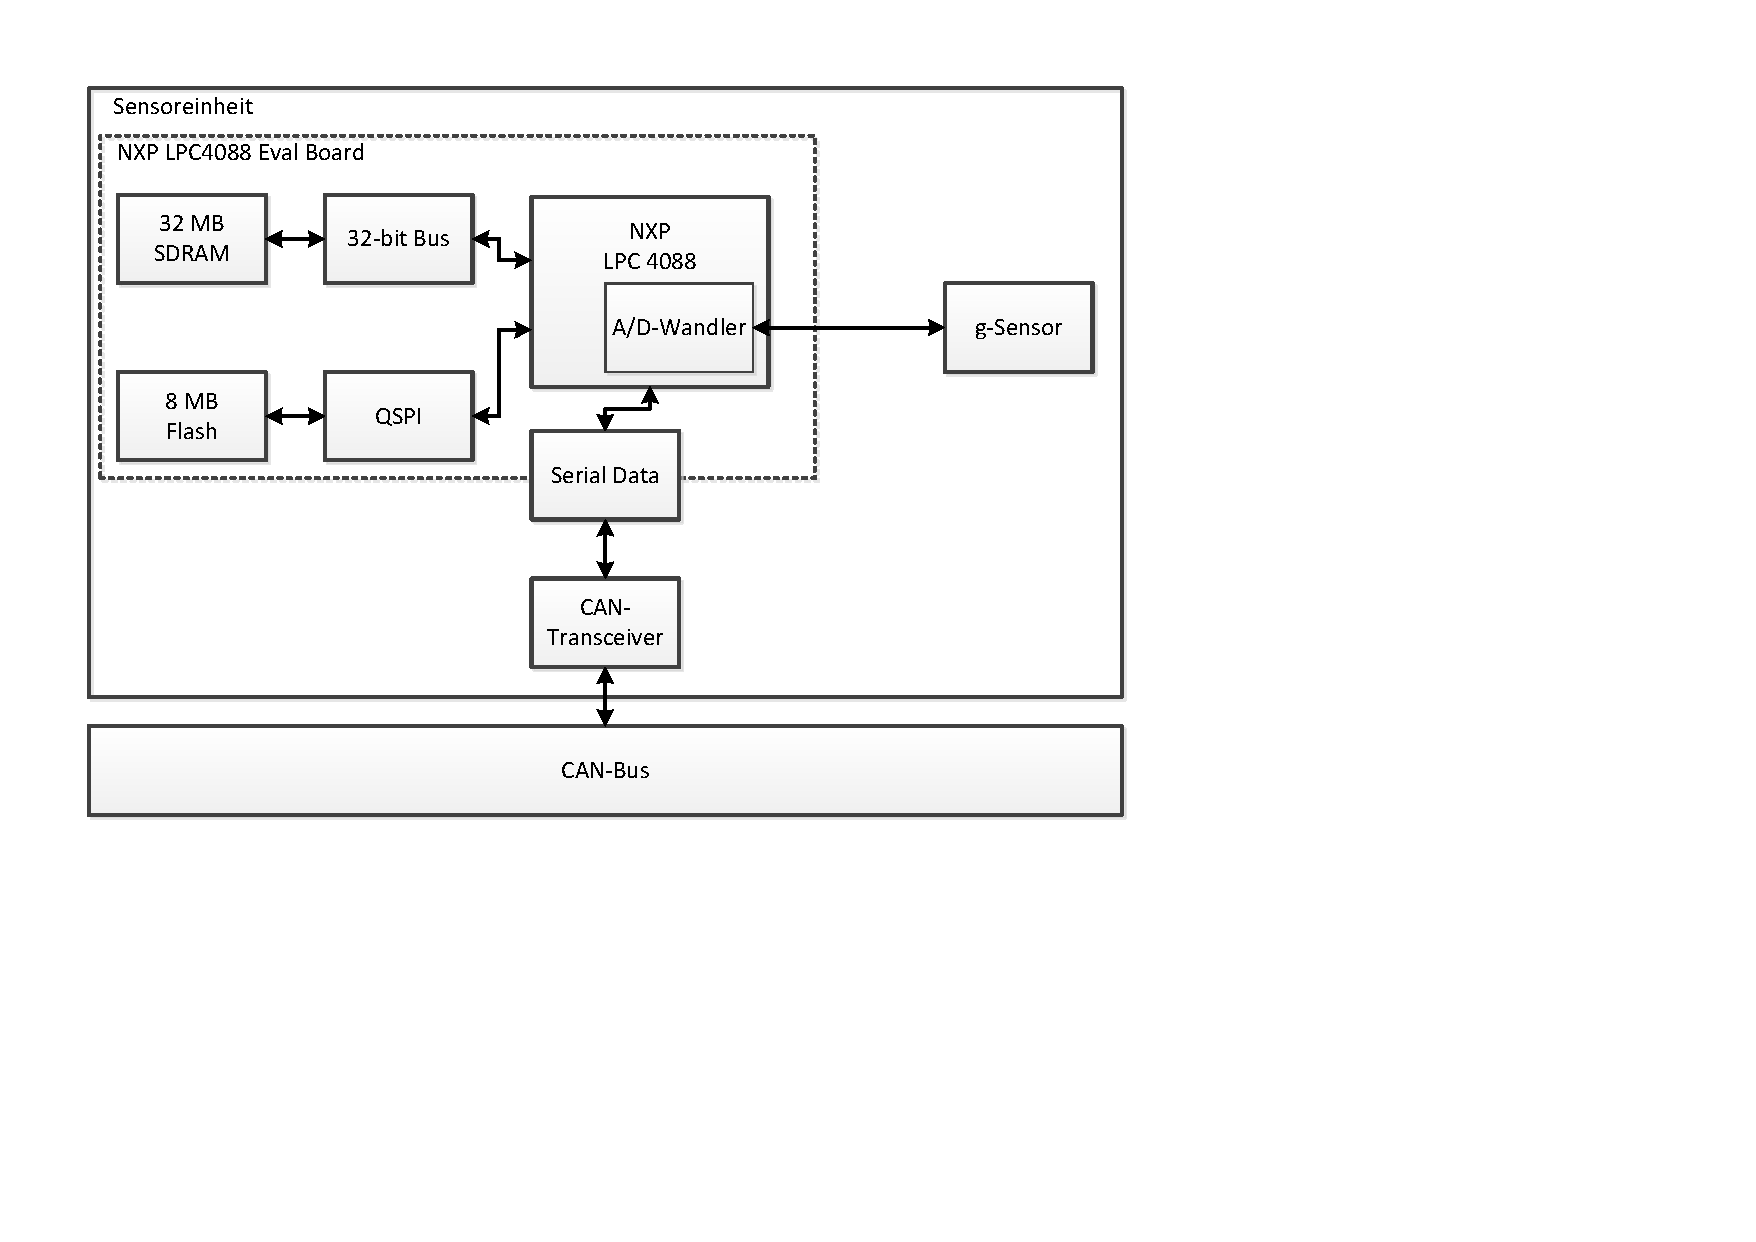
\includegraphics[width=0.8\textwidth]{images/visio/hardware_sensor.pdf}
	\caption{Schematischer Hardware-Aufbau der \gls{sensoreinh}.}
	\label{fig.hw_sensor}
\end{figure}


